\documentclass[11]{beamer}
\usetheme{Warsaw}
\usepackage[utf8]{inputenc}
\usepackage{amsmath}
\usepackage{amsfonts}
\usepackage{amssymb}
\usepackage{color}
\usepackage{siunitx}
%\usepackage[table]{xcolor} 
\usepackage{color, colortbl}

\definecolor{LightCyan}{rgb}{0.88,1,1}
\definecolor{lightgray}{gray}{0.9}
\usepackage{tikz}
\usetikzlibrary{shapes,snakes,arrows,positioning}


% Define box and box title style
\tikzstyle{mybox} = [draw=red, fill=blue!20, very thick,
    rectangle, rounded corners, inner sep=10pt, inner ysep=20pt]
\tikzstyle{fancytitle} =[fill=red, text=white]

\author{Arindam Basu \hspace{5 cm}\newline{arindam@barc.gov.in}}
\title{Accelerator Technology-Vacuum \newline{Vacuum Introduction Part-1}}

%\setbeamercovered{transparent} 
%\setbeamertemplate{navigation symbols}{} 
%\logo{} 
\institute{IADD,BARC} 
%\date{} 
\subject{Accelerator Technology-Vacuum} 
\begin{document}

\begin{frame}
\titlepage
\end{frame}

%\begin{frame}
%\tableofcontents
%\end{frame}





\begin{frame}{Classification of Vacuum}
Vacuum can be classified in three broader categories. These are 
\begin{center}
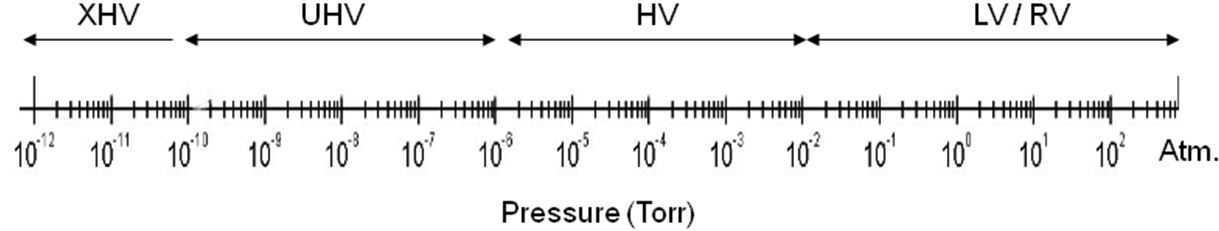
\includegraphics[width=0.5\textwidth]{Vacuum_Scale.png}
\end{center}

\begin{block}{}
	\begin{itemize}
		\item  Rough Vacuum :  759 to $1x 10^{-3}$ Torr
		\item  High Vacuum   :  $1x 10^{-3}$ Torr to $1x 10^{-6}$  Torr
		\item  Ultrahigh Vacuum  :$1x 10^{-6}$  Torr to $1x 10^{-10}$ Torr
		\item  Extra High Vacuum : Less than $1x 10^{-10}$ Torr
	\end{itemize}

\end{block}

\end{frame}





 




\begin{frame}{• Vacuum Establishment}

\begin{exampleblock}

\begin{enumerate}

\item Removal of gas molecules do not happen automatically. To establish vacuum molecules are pumped out of the vacuum system.
\item A vacuum pump is a device which removes gas molecules from the vacuum chamber. 
\item Removal of the gas molecules are done by 
\begin{itemize}
 \item Driving out molecules from the system.
 \item Absorbing molecules in a trap.
 \item Chemically changing the molecules.
\end{itemize}
 
\item Based on these principles different types of vacuum pumps are built.

\end{enumerate}

\end{exampleblock}		


\end{frame}





\begin{frame}{Classification of Vacuum Pumps}
\begin{center}
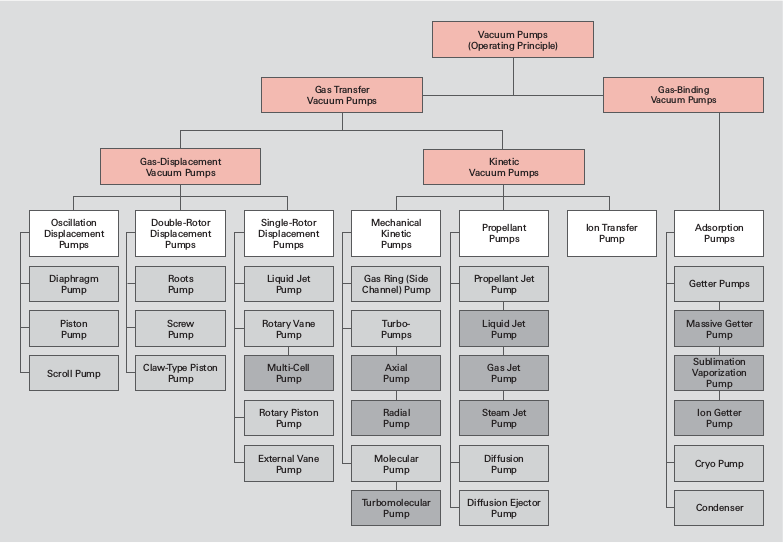
\includegraphics[width=0.9\textwidth]{OverviewOfVacuumPumps.png}
\end{center}
\end{frame}



\begin{frame}{Oil Sealed Rotary Pump}
\begin{center}
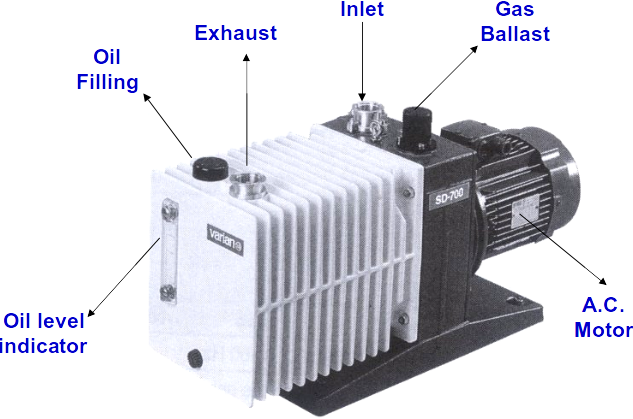
\includegraphics[width=0.8\textwidth]{rotaryPumpMarked.png}
\end{center}
\end{frame}




\begin{frame}{Turbo Molecular Pump}
\begin{center}
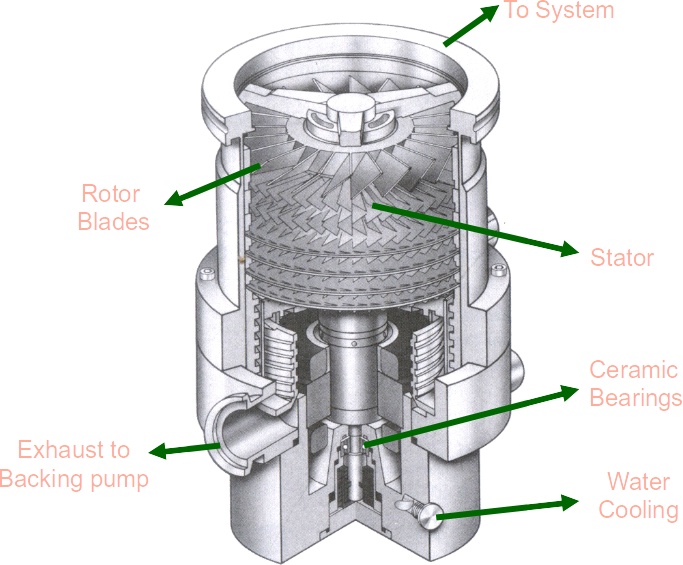
\includegraphics[width=0.8\textwidth]{TurboPump_marked.png}
\end{center}
\end{frame}


\begin{frame}{Turbo Molecular Pump}
\begin{center}
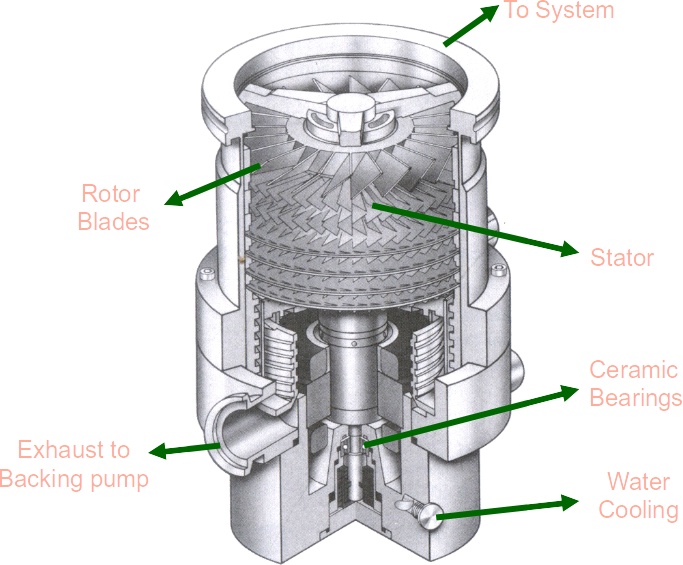
\includegraphics[width=0.3\textwidth]{TurboPump_marked.png}
\end{center}

\begin{itemize}
 \item First made in 1958 from molecular drag pumps
 \item Bladed turbine that compresses gas molecules
 \item High volumetric efficiency for a given size or diameter
 \item Rotor is concentric to the stator
 \item Very high RPM possible due to stable balanced forces
 \item The tips of the rotor blades move with supersonic velocity (600 - 1200 Hz)
 \item  Due to high tip velocity small size is possible
 \item Multistaged can have upto 10 stages,depending on the rotor dia.
\end{itemize}

\end{frame}


\begin{frame}{Turbo Molecular Pump : Pumping Speed Criteria}
Pumping Speed dependent on 
\begin{itemize}
 \item  Type of gas 
  \item     The inlet flange diameter
    \item   The rotor/stator design, 
      \item The RPM  
      \item  Molecular weight of the gas.
 
\end{itemize}
\end{frame}

\begin{frame}{Turbo Molecular Pump : Compression Ratio}
Compression Ratio $K_0$
       always given for a specific gas
       defined as the ratio of the foreline pressure pfl to inlet pressure pin at zero throughput
       relation between the number of pumping stages and $K_0$   
 is given by:

                  $log K_{0} \approx z f \sqrt{M} $\\
       where z - the no. of pumping stages,\\
                    f - the RPM and \\
                   M - molecular wt of the gas.
\end{frame}


\begin{frame}{Turbo Molecular Pump:Pumping Curve}
\begin{center}
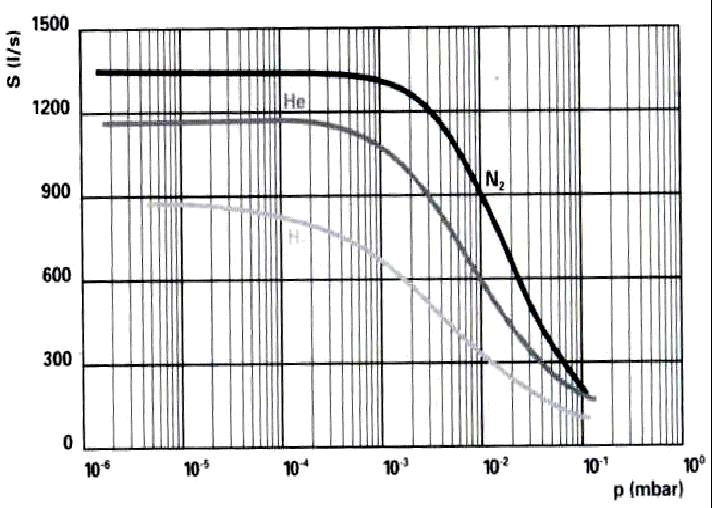
\includegraphics[width=0.8\textwidth]{turboPumpingCurve.png}
\end{center}
\end{frame}

\begin{frame}{Turbo Molecular Pump:Ultimate Pressure}

     \begin{center}
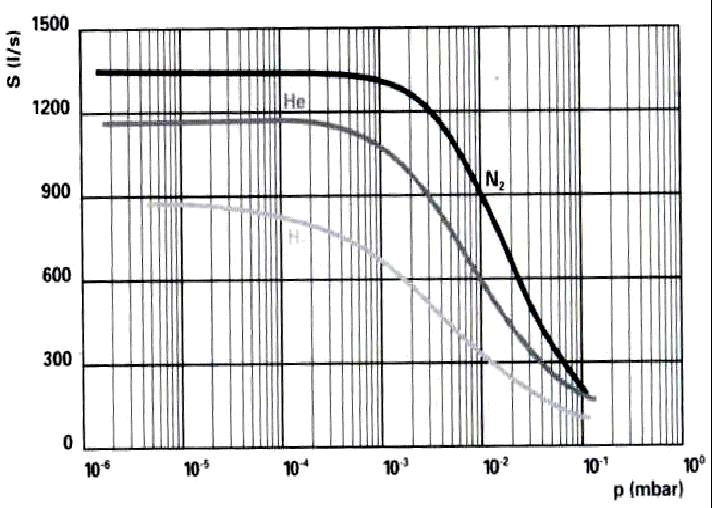
\includegraphics[width=0.3\textwidth]{turboPumpingCurve.png}
\end{center}
     
      \begin{itemize}
       \item Usually of the order of $10^{-9}$ mbar
       \item Depends on the type of forepump and the type of inlet flange seal.
       \end{itemize}
\end{frame}


\begin{frame}{Vacuum Pumps for Various Vacuum Rages}

\begin{enumerate}
\item Pumps for Low vacuum
	\begin{itemize}
	\item Rotary vane pump
    \item    Roots Blowers
     \item   Scroll
      \item  Diaphragm
      \item  Rotary Piston
      \item  Cryo-sorption
     \item   Reciprocating Piston pump
	\end{itemize}
	
\item Pumps for High vacuum
        
        \begin{itemize}
			\item Vapour Diffusion pumps	
    		\item    Turbo Molecular Pump
	    \end{itemize}
	
\item Pumps for Ultra High vacuum
        
        \begin{itemize}
			\item Turbomolecular pump
      		\item 	 Sputter Ion Pump
       		\item 		Cryogenic Pump
       		\item 		Titanium Sublimation pump
       		\item 		NEG Pumps
    		   
	    \end{itemize}


\end{enumerate}


\end{frame}

\begin{frame}{Selection Criteria of a Vacuum Pump}
The following are Main Criteria
\begin{itemize}
 \item Ultimate Vacuum or Order of Vacuum
 \item  Cleanness of Vacuum
 \item Pumping Speed 
 \item Gas Load : Quantity \& Nature
 \item Sensitivity of  Other Instrument(s) 
 \item Cost : Initial, Operating \& Maintenance
\end{itemize}

\end{frame}



\begin{frame}{Types of }

\end{frame}






\begin{frame}

\end{frame}











\begin{frame}

\end{frame}






\begin{frame}

\end{frame}





%\begin{frame}
%\begin{thebibliography}{10}
%\bibitem{Goldbach1742}[Goldbach, 1742]
%Christian Goldbach.
%\newblock A problem we should try to solve \break before the ISPN ’43 deadline,
%\newblock \emph{Letter to Leonhard Euler}, 1742.
%\end{thebibliography}

%\begin{block}{Open Questions}
%Is every even number the sum of two primes?
%\cite{Goldbach1742}
%\end{block}
%\end{frame}









\end{document}